\section*{Run over more than 50 epochs with varied batch
size}

Test report

by E. Marquer, 2018/06/19, Synalp and Université de Lorraine

\subsection{Abstract}

The test is composed of 4 runs on grele, with:
\begin{itemize}
\item bptt 200, batch-size 1
\item bptt 100, batch-size 2
\item bptt 50, batch-size 4
\item bptt 25, batch-size 8
\end{itemize}

Run has been interrupted by an overflow of disk space due to the
detailed logs; next runs will used reduced logs.

Run time per epoch varies from 30 to 7 min.

\subsubsection{Shared parameters}

\begin{longtable}[]{@{}ll@{}}
\hline
parameter & value\tabularnewline
\hline
\endhead
corpus & enwik8reduced\tabularnewline
history\_strategy & layer-constant-length\tabularnewline
max\_history & 25\tabularnewline
bptt & \emph{variable}\tabularnewline
batch\_size & \emph{variable}\tabularnewline
epochs & 4\tabularnewline
lr & 1e-3\tabularnewline
weight\_decay & 1.2e-6\tabularnewline
epochs & 4\tabularnewline
valid\_len & 500,000\tabularnewline
log\_interval & 500\tabularnewline
save\_interval & 500\tabularnewline
memory\_interval & 100\tabularnewline
hidden\_size & 460\tabularnewline
embed\_size & 400\tabularnewline
growth\_factor & 5\tabularnewline
rnn\_type & RNN\tabularnewline
reset\_hidden & False\tabularnewline
reset\_growth & True\tabularnewline
cuda\_on & True\tabularnewline
\hline
\end{longtable}

\subsection{Results}

At the end of each epoch, we see a spike in BPC, due to the first
evaluation of the epoch (BPC is reinitialised to 0, causing a spike).
With any number of batch, while keeping the
\lstinline!bptt * batch_size! ratio, BPC and Validation BPC do not vary.

Even with 200 epochs, with batch size of 1, there is no trace of
over-fitting.

\subsubsection{Epoch run time:}

\begin{longtable}[]{@{}lllll@{}}
\hline
Epoch & Run time b=1 & Run time b=2 & Run time b=4 & Run time
b=8\tabularnewline
\hline
\endhead
1 & 30 min & 21 min & 18 min & 19 min\tabularnewline
10 & 21 min & 14 min & 14 min & 17 min\tabularnewline
15 & 7 min & 7 min & 8 min & 11 min\tabularnewline
\hline
\end{longtable}

\begin{longtable}[]{@{}lll@{}}
\hline
Epoch 1 & Epoch 10 & Epoch 15\tabularnewline
\hline
\endhead
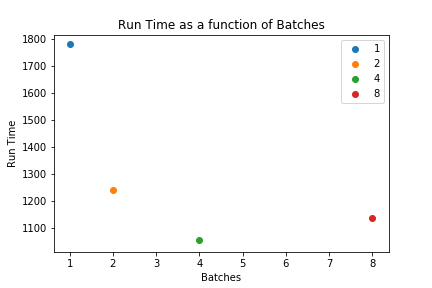
\includegraphics[width=.31\textwidth]{parts/appendix/reports-gmsnn/docs_esteban-latex/test_reports/2018-06-19/b1a8_batch_epoch_1.png} &
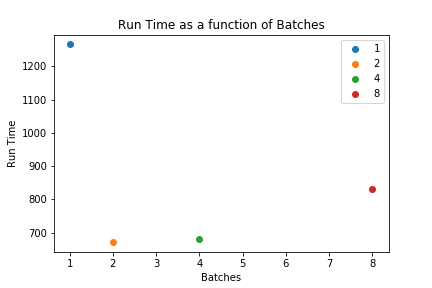
\includegraphics[width=.31\textwidth]{parts/appendix/reports-gmsnn/docs_esteban-latex/test_reports/2018-06-19/b1a8_batch_epoch_10.png} &
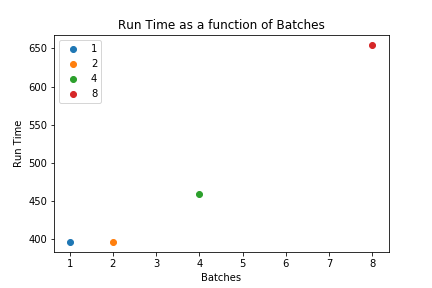
\includegraphics[width=.31\textwidth]{parts/appendix/reports-gmsnn/docs_esteban-latex/test_reports/2018-06-19/b1a8_batch_epoch_15.png}\tabularnewline
\hline
\end{longtable}

Run time can be split over two set of epochs: before, and after the 15th
epoch. Before the 15th epoch, run is faster with more batches, with the
exception of batch-size 8, which is slower than batch-size 2 and 4.
After the 15th epoch, run is slower with more batches.

To optimize run time, it is necessary to balance run time before 15
epochs. If a high number of batches is planed (50),
between 2 and 4 batches are preferable, because the run time after epoch
15 has a lot of impact on global run time; however, if only a few epochs
are planed (20), a high number of batches is preferable, as
run time before epoch 15 is the most important.

With current corpus, 2, 3 or 4 batches are the most interesting setup.

Decrease in run time is most probably due to the history of the upper
layers, that needs multiple epochs to fill.

\subsubsection{Plots}

\paragraph{BPC}

\begin{tabular}{ll}
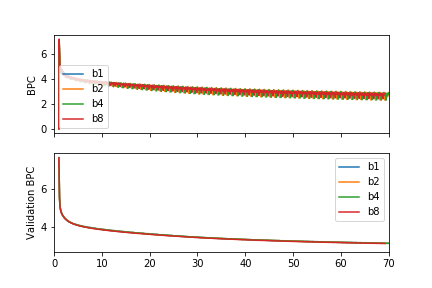
\includegraphics[width=.45\textwidth]{parts/appendix/reports-gmsnn/docs_esteban-latex/test_reports/2018-06-19/b1a8_frac.png}
&
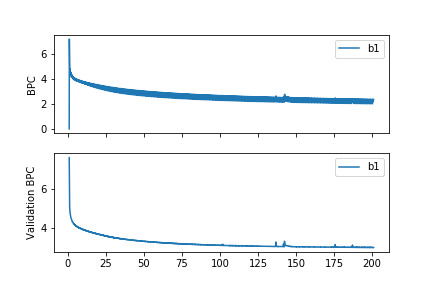
\includegraphics[width=.45\textwidth]{parts/appendix/reports-gmsnn/docs_esteban-latex/test_reports/2018-06-19/b1a8_200.png}
\end{tabular}

\paragraph{Memory}

\begin{figure}[H]
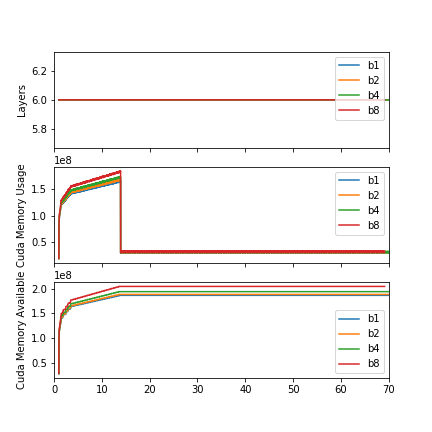
\includegraphics[width=.8\textwidth]{parts/appendix/reports-gmsnn/docs_esteban-latex/test_reports/2018-06-19/b1a8_memory.png}
\end{figure}

\paragraph{Run time (in seconds)}

\begin{figure}[H]
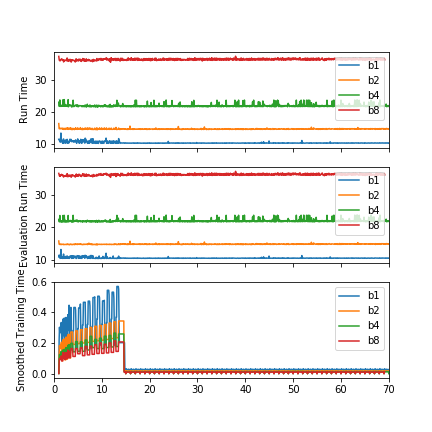
\includegraphics[width=.8\textwidth]{parts/appendix/reports-gmsnn/docs_esteban-latex/test_reports/2018-06-19/b1a8_time.png}
\end{figure}

\subparagraph{Epoch run time}

\begin{figure}[H]
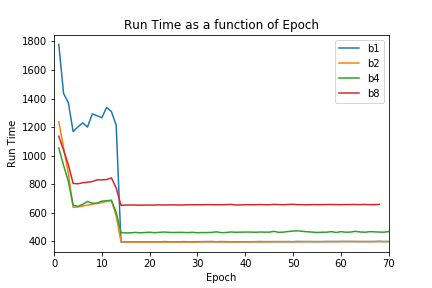
\includegraphics[width=.8\textwidth]{parts/appendix/reports-gmsnn/docs_esteban-latex/test_reports/2018-06-19/b1a8_epoch.png}
\end{figure}

\subsection{Next steps}

\begin{itemize}
\item
  Independent impact of batch number and sequence length:

  \begin{itemize}
  \item
    Run with fixed batch number and varying sequence length
  \item
    Run with fixed sequence length and varying batch number
  \end{itemize}
\item
  Impact of corpus length on optimal number of batch and sequences:

  \begin{itemize}
  \item
    Run with varying sequence length and varying batch number over the
    full length corpus
  \end{itemize}
\item
  Number of parameters:

  \begin{itemize}
  \item
    Increase the hidden layer size
  \end{itemize}
\item
  {[}Future{]} Transmission rate impact:

  \begin{itemize}
  \item
    Compare optimal values of parameters, and BPC reached with varying
    transmission rate
  \end{itemize}
\end{itemize}
